\documentclass{article}
\usepackage[utf8]{inputenc}
%\usepackage{graphicx} % Required for inserting images
\usepackage{pgfplots}
\pgfplotsset{compat=1.18, width=10cm}

\title{pgfplots Test}
\author{Isaac Tavera}
\date{Noviembre del 2023}

\begin{document}

\section{Introduction}

\begin{tikzpicture}
    \begin{axis}[xmin=-2, xmax=2, ymin=-1, ymax=2, axis lines=middle,]
        \addplot[color=black, samples=100]{x^2};
    \end{axis}
\end{tikzpicture}
\newline
Una gráfica cuadrática: \newline
\begin{tikzpicture}
    \begin{axis}[xmin=-2, xmax=2, ymin=-2.5, ymax=2.5, axis lines=middle, xlabel=$x$, ylabel=$y$, title={Test Title}, xtick={-1.5, -1, -0.5, 0.5, 1, 1.5}]
        \addplot[color=black, dashed, mark=*, samples=50]{x^2};
        \addplot[color=blue, samples=100, domain=-1:1]{1-x^2};
        \addplot[color=blue, samples=100, domain=-2:-1.5]{1-x^2};
        \addplot[color=blue, samples=100, domain=1.5:2]{1-x^2};
        \end{axis}
\end{tikzpicture}
\newline
Otra gráfica cuadrática: \newline
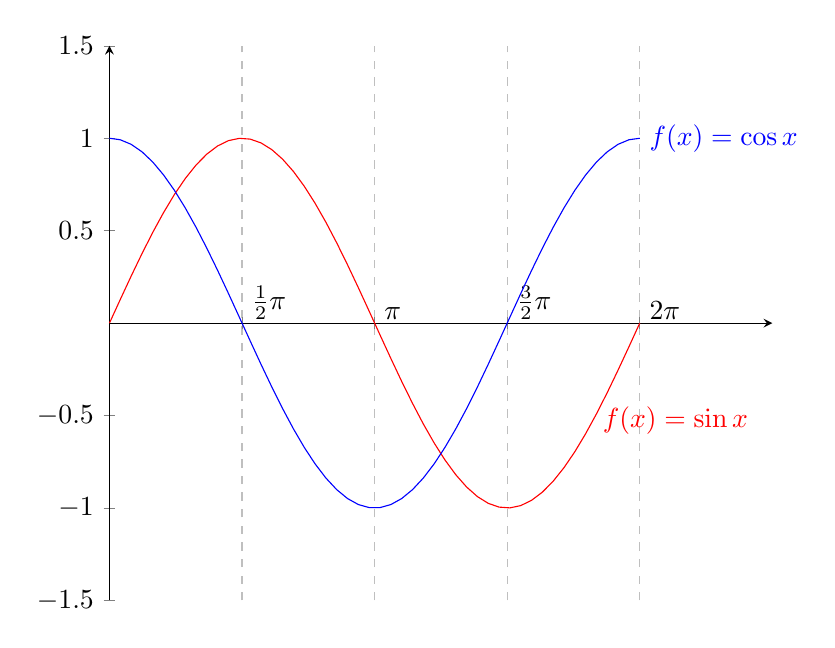
\begin{tikzpicture}
    \begin{axis}[clip=false, xmin=0, xmax=2.5*pi, ymin=-1.5, ymax=1.5, axis lines=middle, xtick={0,pi/2, pi, 3*pi/2, 2*pi}, xticklabels={$0$, $\frac{1}{2}\pi$, $\pi$, $\frac{3}{2}\pi$, $2\pi$},xticklabel style={anchor=south west}, xmajorgrids=true, grid style=dashed]
        \addplot[domain=0:2*pi, color=red, samples=50]{sin(deg(x))}node[right,pos=0.9]{$f(x)=\sin x$};
        \addplot[domain=0:2*pi, color=blue, samples=50]{cos(deg(x))}node[right,pos=1]{$f(x)=\cos x$};
    \end{axis}
\end{tikzpicture}

\end{document}
